\section{Results for Einstein Vacuum Equations}

We test the vacuum iteration in five regimes of increasing geometric and
numerical difficulty.  The first three experiments admit explicit reference
metrics and therefore measure the error directly by comparing the computed
section metric with the exact one.  The last two experiments evolve genuinely
nonspherical characteristic data, for which no explicit spacetime is
available; there we report a positive norm of the first-order Ricci residual
on a protected interior region, together with metric--connection consistency
checks.  The residual is evaluated from the stored weighted connection
variables and fresh derivatives, with the audit grid specified for each case.  This avoids
second null derivatives of the metric and the potentially singular derivative
$\nabla_4\chih$ at the initial corner; intrinsic angular curvature uses the
smooth sphere data.  These diagnostics assess the numerical equations and do
not furnish a certified metric-error bound.

\subsection{Regular Schwarzschild and Kerr benchmarks}

We begin with the Schwarzschild and subextremal Kerr families.  In
Schwarzschild coordinates, the metric of mass $M>0$ is
\begin{equation}\label{eq:results-schwarzschild-static}
  \bg_{\mathrm{Sch}}
  =-\left(1-\frac{2M}{r}\right)\dd t^2
   +\left(1-\frac{2M}{r}\right)^{-1}\dd r^2
   +r^2\left(\dd\vartheta^2+\sin^2\vartheta\,\dd\varphi^2\right).
\end{equation}
Let
\begin{equation}
  r_*=r+2M\log\left(\frac{r}{2M}-1\right)+C,
  \qquad t=u+v,\qquad r_*=v-u,
\end{equation}
where the additive constant $C$ fixes the reference sphere.  Then
\eqref{eq:results-schwarzschild-static} becomes
\begin{equation}\label{eq:results-schwarzschild-double-null}
  \bg_{\mathrm{Sch}}
  =-4\Omega^2\dd u\dd v+\slg_{AB}\dd\theta^A\dd\theta^B,
  \qquad
  \Omega^2=1-\frac{2M}{r},\qquad
  \slg=r^2\roundg,\qquad b=0,
\end{equation}
with $r=r(v-u)$.  Thus the Schwarzschild benchmark is already in the
double-null gauge used by the iteration.

For Kerr, write $a$ for the angular momentum per unit mass and set
\begin{equation}
  \rho^2=r^2+a^2\cos^2\vartheta,\qquad
  \Delta=r^2-2Mr+a^2.
\end{equation}
The Boyer--Lindquist expression is
\begin{align}\label{eq:results-kerr-bl}
  \bg_{\mathrm K}={}&
  -\left(1-\frac{2Mr}{\rho^2}\right)\dd t^2
  -\frac{4Mar\sin^2\vartheta}{\rho^2}\dd t\dd\varphi
  +\frac{\rho^2}{\Delta}\dd r^2+\rho^2\dd\vartheta^2 \notag\\
  &+\frac{\sin^2\vartheta}{\rho^2}
  \left((r^2+a^2)^2-a^2\Delta\sin^2\vartheta\right)\dd\varphi^2.
\end{align}
To put \eqref{eq:results-kerr-bl} into double-null form, we use the optical
coordinates $(u,v,\vartheta_*,\varphi_*)$ defined by
\begin{equation}\label{eq:results-kerr-coordinate-map}
  t=u+v,\qquad s=u-v,\qquad
  r=r(s,\vartheta_*),\qquad
  \vartheta=\vartheta(s,\vartheta_*),\qquad
  \varphi=\varphi_*+h(s,\vartheta_*).
\end{equation}
The functions $r$, $\vartheta$, and $h$ are obtained from the Kerr optical
map, with $r=4M$, $\vartheta=\vartheta_*$, and $h=0$ on the reference
two-sphere.  If $\widetilde g_{\alpha\beta}$ denotes the pullback of
\eqref{eq:results-kerr-bl} under \eqref{eq:results-kerr-coordinate-map}, the
optical equations give
\begin{equation}
  \widetilde g_{vv}=0,\qquad \widetilde g_{vA}=0,\qquad
  \widetilde g_{uu}=\slg_{AB}b^Ab^B.
\end{equation}
Consequently the pulled-back metric is exactly
\begin{align}\label{eq:results-kerr-double-null}
  \bg_{\mathrm K}
  &=-4\Omega^2\dd u\dd v
   +\slg_{AB}(\dd\theta^A-b^A\dd u)
                  (\dd\theta^B-b^B\dd u), \notag\\
  \Omega^2&=-\frac12\widetilde g_{uv},\qquad
  \slg_{AB}=\widetilde g_{AB},\qquad
  b^A=-\slg^{AB}\widetilde g_{uB}.
\end{align}

All runs use $M=1$.  We take $a=0,0.3,0.7,0.9$ and solve on the short
rectangle
\begin{equation}
  -1\leq u\leq-\frac12,\qquad 0\leq v\leq\frac12,
\end{equation}
and on the long rectangle
\begin{equation}
  -1\leq u\leq0,\qquad 0\leq v\leq1.
\end{equation}
The coordinate refinements contain $17^2$, $33^2$, and $65^2$ nodes.  The
Schwarzschild runs use 50 spherical points with retained degree five, while
the finest Kerr results below use 86 spherical points with retained degree
seven.  Eight complete Picard sweeps are used in every case.

Because the exact metrics are known, no curvature differentiation is needed
to define the primary error.  At every angular and double-null grid point
$q=(\theta,u_i,v_j)$, set
\begin{equation}\label{eq:results-exp1-metric-error}
  E_g(q)=\left\lVert
  \slg_{\mathrm{num}}(q)-\slg_{\mathrm{exact}}(q)
  \right\rVert_{\mathrm F},
\end{equation}
where $\norm{\cdot}_{\mathrm F}$ is the Frobenius norm in the pole-free
ambient representation of tangent two-tensors.  Table
\ref{tab:results-exp1-metric-error} gives the median and arithmetic mean of
$E_g$ over all points of each $65\times65$ run.  Schwarzschild and the
zero-spin Kerr control agree with the explicit metric essentially to
floating-point accuracy.  For $a\neq0$, the larger error is associated with
the numerical angular reconstruction of the Kerr optical map; it remains of
order $10^{-6}$ in the mean for all rotating cases considered here.

\begin{table}[htbp]
  \centering
  \caption{Final section-metric error \eqref{eq:results-exp1-metric-error} on
  the finest coordinate grid.}
  \label{tab:results-exp1-metric-error}
  \begin{tabular}{llrrr}
    \toprule
    Family & Domain & $\operatorname{median} E_g$
      & $\operatorname{mean} E_g$ & $\max E_g$ \\
    \midrule
    \TableRows{tables/exp01-rows.tex}
    \bottomrule
  \end{tabular}
\end{table}

\subsection{Schwarzschild horizon in static and Kruskal coordinates}

The second experiment keeps the Schwarzschild geometry
\eqref{eq:results-schwarzschild-static} fixed and changes only the coordinate
system.  It separates loss of numerical conditioning caused by a degenerating
chart from the regular geometry of the event horizon.  In the static
double-null chart \eqref{eq:results-schwarzschild-double-null}, the additive
constant in $r_*$ is chosen so that
\begin{equation}
  r=2M(1+\epsilon)
  \quad\text{at}\quad v-u=\frac12 .
\end{equation}
The four offsets
\begin{equation}
  \epsilon=10^{-1},\ 10^{-2},\ 10^{-4},\ 10^{-6}
\end{equation}
therefore give
\begin{equation}
  \min\Omega^2=\frac{\epsilon}{1+\epsilon}.
\end{equation}
Although every one of these rectangles remains in the exterior $r>2M$, the
last case places the closest numerical sphere only $2M\epsilon=2\times10^{-6}$
from the horizon when $M=1$.  The lapse consequently becomes small and the
static coordinate representation becomes increasingly ill-conditioned.

For the horizon-crossing test, define shifted Kruskal coordinates
\begin{equation}
  U=u+\frac34,\qquad V=v+1.
\end{equation}
The relation between $r$ and $(U,V)$ and the corresponding double-null metric
are
\begin{equation}\label{eq:results-kruskal-double-null}
  UV=\left(1-\frac{r}{2M}\right)e^{r/(2M)},\qquad
  \bg_{\mathrm{Sch}}
  =-\frac{32M^3}{r}e^{-r/(2M)}\dd U\dd V+r^2\roundg,
\end{equation}
or, in the notation of this paper,
\begin{equation}
  \Omega^2=\frac{8M^3}{r}e^{-r/(2M)},\qquad
  \slg=r^2\roundg,\qquad b=0.
\end{equation}
Unlike the static lapse, this $\Omega$ is positive and regular at $r=2M$.
The principal Lambert branch gives the explicit inversion
\begin{equation}
  r=2M\left[1+
  W_0\left(-\frac{UV}{e}\right)\right].
\end{equation}

All five cases are solved on the same numerical rectangle
\begin{equation}\label{eq:results-exp2-domain}
  -1\leq u\leq-\frac12,\qquad 0\leq v\leq\frac12,
\end{equation}
using $17^2$, $33^2$, and $65^2$ coordinate grids, 50 spherical points,
retained angular degree five, and eight Picard sweeps.  For the Kruskal case,
\eqref{eq:results-exp2-domain} corresponds to
\begin{equation}
  -\frac14\leq U\leq\frac14,\qquad
  1\leq V\leq\frac32.
\end{equation}
It crosses the future event horizon $U=0$ and covers
$1.67549\leq r\leq2.24420$ for $M=1$.

We again use the direct metric error $E_g$ defined in
\eqref{eq:results-exp1-metric-error}.  Table
\ref{tab:results-exp2-metric-error} reports its median and arithmetic mean on
the finest grid.  The static-coordinate metric itself is reproduced to
roundoff even as $\Omega^2$ approaches zero.  The Kruskal calculation also
remains highly accurate across the horizon, with a mean section-metric error
of $1.12\times10^{-12}$.  The supplementary curvature checks use first null derivatives of the
weighted connection variables, with the metric--connection consistency
reported separately.
Derivative-based curvature diagnostics are more sensitive to the static lapse
degeneration; this is a coordinate-conditioning effect and does not indicate
a curvature singularity at $r=2M$.

\begin{table}[htbp]
  \centering
  \caption{Final section-metric error for the Schwarzschild horizon tests on
  the $65\times65$ coordinate grid.}
  \label{tab:results-exp2-metric-error}
  \begin{tabular}{lrrr}
    \toprule
    Coordinates & $\operatorname{median} E_g$
      & $\operatorname{mean} E_g$ & $\max E_g$ \\
    \midrule
    \TableRows{tables/exp02-rows.tex}
    \bottomrule
  \end{tabular}
\end{table}


\subsection{Schwarzschild interior and approach to \texorpdfstring{\(r=0\)}{r=0}}

The third experiment uses the Schwarzschild solution in the regular Kruskal
form \eqref{eq:results-kruskal-double-null}, now entirely inside the event
horizon.  We shift the Kruskal coordinates by
\begin{equation}
  U=u+2,\qquad V=v+\frac15,
\end{equation}
and use the same relation
\begin{equation}
  UV=\left(1-\frac{r}{2M}\right)e^{r/(2M)}.
\end{equation}
The singular boundary $r=0$ corresponds to $UV=1$.  To approach it without
including it, let
\begin{equation}
  x_\epsilon=(1-\epsilon)e^\epsilon,\qquad
  v_0(u)=\frac{x_\epsilon}{u+2}-\frac15,
\end{equation}
and introduce a fixed computational coordinate $\xi$ through
\begin{equation}\label{eq:results-exp3-map}
  v=\xi v_0(u).
\end{equation}
The numerical domain is therefore the curved characteristic region
\begin{equation}\label{eq:results-exp3-domain}
  -1\leq u\leq-\frac12,\qquad
  0\leq\xi\leq1,\qquad
  0\leq v\leq v_0(u).
\end{equation}
On its future boundary $\xi=1$ one has
\begin{equation}
  UV=x_\epsilon,\qquad r=2M\epsilon.
\end{equation}
We take
\begin{equation}
  \epsilon=2^{-1},2^{-2},\ldots,2^{-6}.
\end{equation}
For $M=1$, the six future boundaries thus lie at
$r=1,1/2,1/4,1/8,1/16,1/32$.  The opposite characteristic face has
$r\leq1.84064$, so every case lies strictly within the Schwarzschild event
horizon.

The map \eqref{eq:results-exp3-map} is discretized with tensor-product
Chebyshev--Lobatto grids containing $17^2$, $33^2$, and $49^2$ points.  The
physical derivatives include both Jacobian terms generated by the
$u$-dependence of $v_0$.  Each case receives at most 20 Picard sweeps.  If an
undamped update would make the radius nonpositive, dyadic backtracking chooses
the largest positive, nonincreasing update.  This stabilization prevents an
algebraic breakdown, but it does not by itself establish convergence or
accuracy near $r=0$.

Since the solution is spherically symmetric,
\begin{equation}
  \slg_{\mathrm{num}}=r_{\mathrm{num}}^2\roundg,\qquad
  \slg_{\mathrm{exact}}=r_{\mathrm{exact}}^2\roundg.
\end{equation}
Accordingly, the pointwise metric error
\eqref{eq:results-exp1-metric-error} reduces to
\begin{equation}\label{eq:results-exp3-metric-error}
  E_g=\sqrt{2}\,
  \left|r_{\mathrm{num}}^2-r_{\mathrm{exact}}^2\right|,
\end{equation}
because $\norm{\roundg}_{\mathrm F}=\sqrt2$ in the pole-free ambient
representation.  Table \ref{tab:results-exp3-metric-error} reports the
statistics of \eqref{eq:results-exp3-metric-error} on the $49^2$ grid.

\begin{table}[htbp]
  \centering
  \caption{Final section-metric error in the Schwarzschild-interior
  experiment.  Here $r_{\mathrm{end}}=2M\epsilon$ is the exact radius of the
  future boundary and $M=1$.}
  \label{tab:results-exp3-metric-error}
  \begin{tabular}{ccrrr}
    \toprule
    $\epsilon$ & $r_{\mathrm{end}}$
      & $\operatorname{median}E_g$ & $\operatorname{mean}E_g$ & $\max E_g$ \\
    \midrule
    \TableRows{tables/exp03-rows.tex}
    \bottomrule
  \end{tabular}
\end{table}

The first two future boundaries retain small absolute metric error.  Beginning
at $\epsilon=2^{-3}$, however, the iteration does not settle within 20 sweeps
and the error grows rapidly under further approach to the singularity.  In the
closest case, the exact minimum radius is $1/32$, whereas the computed minimum
is $0.08127$; the maximum relative radius error is $16.43$, and the maximum
relative section-metric error is $3.03\times10^2$.  That case also requires a
dyadic relaxation factor as small as $1/32$.  These results demonstrate the
current method's loss of accuracy near $r=0$; the stabilized finite output is
not evidence of convergence at the Schwarzschild singularity.


\subsection{Strong outgoing short pulse and zero control}

The fourth experiment leaves the class of explicit solutions.  At the corner
we prescribe the round section metric, unit lapse, vanishing shift and
torsion, and the Minkowski expansions,
\begin{equation}
  \begin{aligned}
    \slg(-1,0)&=\roundg,& \Omega(-1,0)&=1,&
    b(-1,0)&=0,& \zeta(-1,0)&=0,\\
    (\Omega\tr\chi)(-1,0)&=2,&
    (\Omega\tr\chib)(-1,0)&=-2.&&
  \end{aligned}
\end{equation}
On the outgoing initial hypersurface, a low-band trace-free tensor is formed
from two polynomial hemisphere tensors $X_+$ and $X_-$ and two disjoint
profiles $q_+$ and $q_-$:
\begin{equation}\label{eq:results-exp4-pulse}
  \Omega\chih(-1,v)
  =\mathcal T_{q_+(v)X_++q_-(v)X_-}[\slg(-1,v)].
\end{equation}
Here $q_+$ has the admissible square-root behavior at $v=0$, $q_-$ is a
smooth interior bump, and both are calibrated on $0\leq v\leq1/2$ so that
the hemisphere integral has strength one after division by $3.2$.  Only the
leading part of this pulse is evolved, on the rectangle
\begin{equation}
  -1\leq u\leq-\frac12,\qquad 0\leq v\leq0.005.
\end{equation}
The zero control uses the identical construction and discretization with
$q_+=q_-=0$.

The perturbation in the strong run is not numerically negligible.  Using the
computed metric and area form, we measure
\begin{equation}
  \norm{\chih(-1,0.005)}_{L^2(S,\slg)}
  =\left(\int_{S_{-1,0.005}}
      \abs{\Omega^{-1}\Omega\chih}_{\slg}^{2}\,
      \dd\mu_{\slg}\right)^{1/2}
  =3.75480,
\end{equation}
while the pointwise maximum is $1.26734$.  Thus the good residual reported
below is not a consequence of evolving an effectively zero datum.

We use $17$ nodes in the logarithmic coordinate $\tau=-\log(-u)$ and $33$
nodes in $s=\sqrt{2v}$, distributed over two and four degree-eight elements,
respectively.  The angular discretization has $550$ sphere points, retained
degree $L=10$, work degree $W=20$, and differentiation degree $D=21$.  Both
runs complete six Picard sweeps.  Since no explicit spacetime is available,
the accuracy statistic is the $L^\infty_{u,v}L^2(S)$ norm of the independently
differentiated first-order Ricci residual on the stencil-protected interior.
The audit transfers scalar, vector, and tensor fields in their typed harmonic
spaces through degree 20 onto 562 sphere points, and raises each coordinate
element degree by three. The protected metric--connection component defects
are $1.75\times10^{-9}$ in the incoming direction and
$2.77\times10^{-7}$ in the outgoing direction.

\begin{table}[htbp]
  \centering
  \caption{Iteration update and independent Ricci residual for the strong
  outgoing pulse and its zero control.  The pointwise column is the maximum
  sphere-point residual on the same protected region.}
  \label{tab:results-exp4-residual}
  \begin{tabular}{lrrr}
    \toprule
    Data & final update & $L^\infty_{u,v}L^2(S)$
      & protected pointwise maximum \\
    \midrule
    \TableRows{tables/exp04-rows.tex}
    \bottomrule
  \end{tabular}
\end{table}

Every boundary spectral-deferred-correction element is accepted.  For the
strong pulse, the maximum collocation and overgrid boundary defects are
$6.36\times10^{-16}$ and $1.47\times10^{-8}$, respectively.  In the zero
control, moving the residual mask farther from the short-pulse endpoint
reduces the $L^\infty_{u,v}L^2(S)$ residual from $1.973\times10^{-9}$ to
$1.737\times10^{-9}$. The exact Minkowski control has the same numerical
floor, $1.973\times10^{-9}$.  The contrast between this numerical floor and the
strong-pulse value isolates the error associated with evolving the
nonspherical datum.


\subsection{Crossed characteristic shears}

The fifth experiment prescribes nonspherical shears on both initial null
hypersurfaces.  Let
\begin{equation}
  A_1=\operatorname{diag}\left(-\frac12,-\frac12,1\right),\qquad
  A_2=\operatorname{diag}(1,-1,0),\qquad
  f_j(n)=n^{\mathsf T}A_jn,
\end{equation}
and define the explicitly normalized round-sphere tensors
\begin{equation}
  X_1=\frac{\sqrt2}{3}\,\tf\nabla^2 f_1,
  \qquad
  X_2=\frac{1}{2\sqrt2}\,\tf\nabla^2 f_2.
\end{equation}
If $\mathcal T_X[\slg]$ denotes the symmetric transfer of $X$ to $\slg$
followed by removal of its $\slg$-trace, the prescribed data are
\begin{equation}\label{eq:results-exp5-shears}
  \Omega\chih(-1,v)=v^{1/2}\mathcal T_{X_1}[\slg(-1,v)],
  \qquad
  \Omega\chibh(u,0)=(u+1)^{1/2}
     \mathcal T_{X_2}[\slg(u,0)].
\end{equation}
At the corner, $\slg=\roundg$, $\Omega=1$, $\Omega\tr\chi=2$,
$\Omega\tr\chib=-2$, and $\zeta=0$.  The lapse is one on both initial
faces and $b(u,0)=0.1\,\partial_\varphi$; the remaining face data are obtained
from the characteristic constraints.

Although the shears in \eqref{eq:results-exp5-shears} vanish continuously at
the corner, the corresponding initial curvature is singular.  The outgoing
shear equation contains $\nabla_4\chih$ and the incoming shear equation
contains $\nabla_3\chibh$.  Their leading transverse derivatives satisfy
\begin{equation}
  \nabla_4\chih=O(v^{-1/2}),\qquad
  \nabla_3\chibh=O((u+1)^{-1/2}).
\end{equation}
Consequently, both $R_{4A4B}$ on $u=-1$ and $R_{3A3B}$ on $v=0$ are
unbounded and hence infinite at the corner in the limiting sense.  This is a
singularity of the prescribed initial curvature, not a large-amplitude
divergence of the shears themselves.  Indeed, at the opposite endpoints of
the two initial faces,
\begin{equation}
  \norm{\chih(-1,\tfrac12)}_{L^2(S,\slg)}=2.727749,
  \qquad
  \norm{\chibh(-\tfrac12,0)}_{L^2(S,\slg)}=0.785641.
\end{equation}

The solution region is the full rectangle
\begin{equation}
  -1\leq u\leq-\frac12,\qquad 0\leq v\leq\frac12.
\end{equation}
We discretize the square-root coordinates
$t=\sqrt{2(u+1)}$ and $s=\sqrt{2v}$ using six degree-ten elements in each
direction, giving a $61\times61$ coordinate grid.  The angular calculation
uses $300$ points with $L=8$, $W=14$, and $D=15$.  The evolution proceeds in
six successive $v$-slabs.  Their terminal weighted updates are
\begin{equation}
  (1.850,\ 4.897,\ 8.694,\ 4.404,\ 6.984,\ 4.761)\times10^{-9},
\end{equation}
all below the prescribed $10^{-8}$ tolerance.

\begin{table}[htbp]
  \centering
  \caption{Aggregate Ricci residual for the crossed-shear experiment.}
  \label{tab:results-exp5-residual}
  \begin{tabular}{lrrrr}
    \toprule
    Region & Number of sections
      & $\operatorname{median}E_{\mathrm{Ric}}$
      & $\operatorname{mean}E_{\mathrm{Ric}}$
      & $\max E_{\mathrm{Ric}}$ \\
    \midrule
    \TableRows{tables/exp05-rows.tex}
    \bottomrule
  \end{tabular}
\end{table}

Let $E_{\mathrm{Ric}}(u,v)$ denote the sum of the sectionwise $L^2(S_{u,v})$
norms of the six weighted Ricci quantities listed in the curvature-residue
subsection.  Table \ref{tab:results-exp5-residual} compares this aggregate
residual on the protected mask with the same statistic on the open
coordinate grid, excluding the four outer endpoint lines.




The protected mask is constructed separately in the two characteristic
coordinates.  In each coordinate it removes the complete first and last
spectral elements and three LGL nodes on each side of every remaining
element interface.  The two-dimensional mask is the tensor product of these
one-dimensional masks, leaving $12$ retained nodes in each direction and
hence $144$ sections.  Its purpose is to omit locations at which the
independent derivative reconstruction encounters the square-root endpoint,
a terminal one-sided boundary, or an element interface; the open-grid row retains the nearby endpoint layers and element interfaces,
but excludes the endpoint lines themselves.  The minimum section-metric eigenvalue is
$2.938\times10^{-2}$, and all immutable characteristic traces are restored
to roundoff, with maximum incoming $\Omega\tr\chi$ mismatch
$1.78\times10^{-15}$.  On the protected mask the metric--connection
defects $\partial_u g+\Lie_b g-2\Omega\chib$ and
$\partial_v g-2\Omega\chi$ have maximum absolute ambient components
$3.10\times10^{-4}$ and $1.85\times10^{-5}$, respectively.

\begin{figure}[htbp]
  \centering
  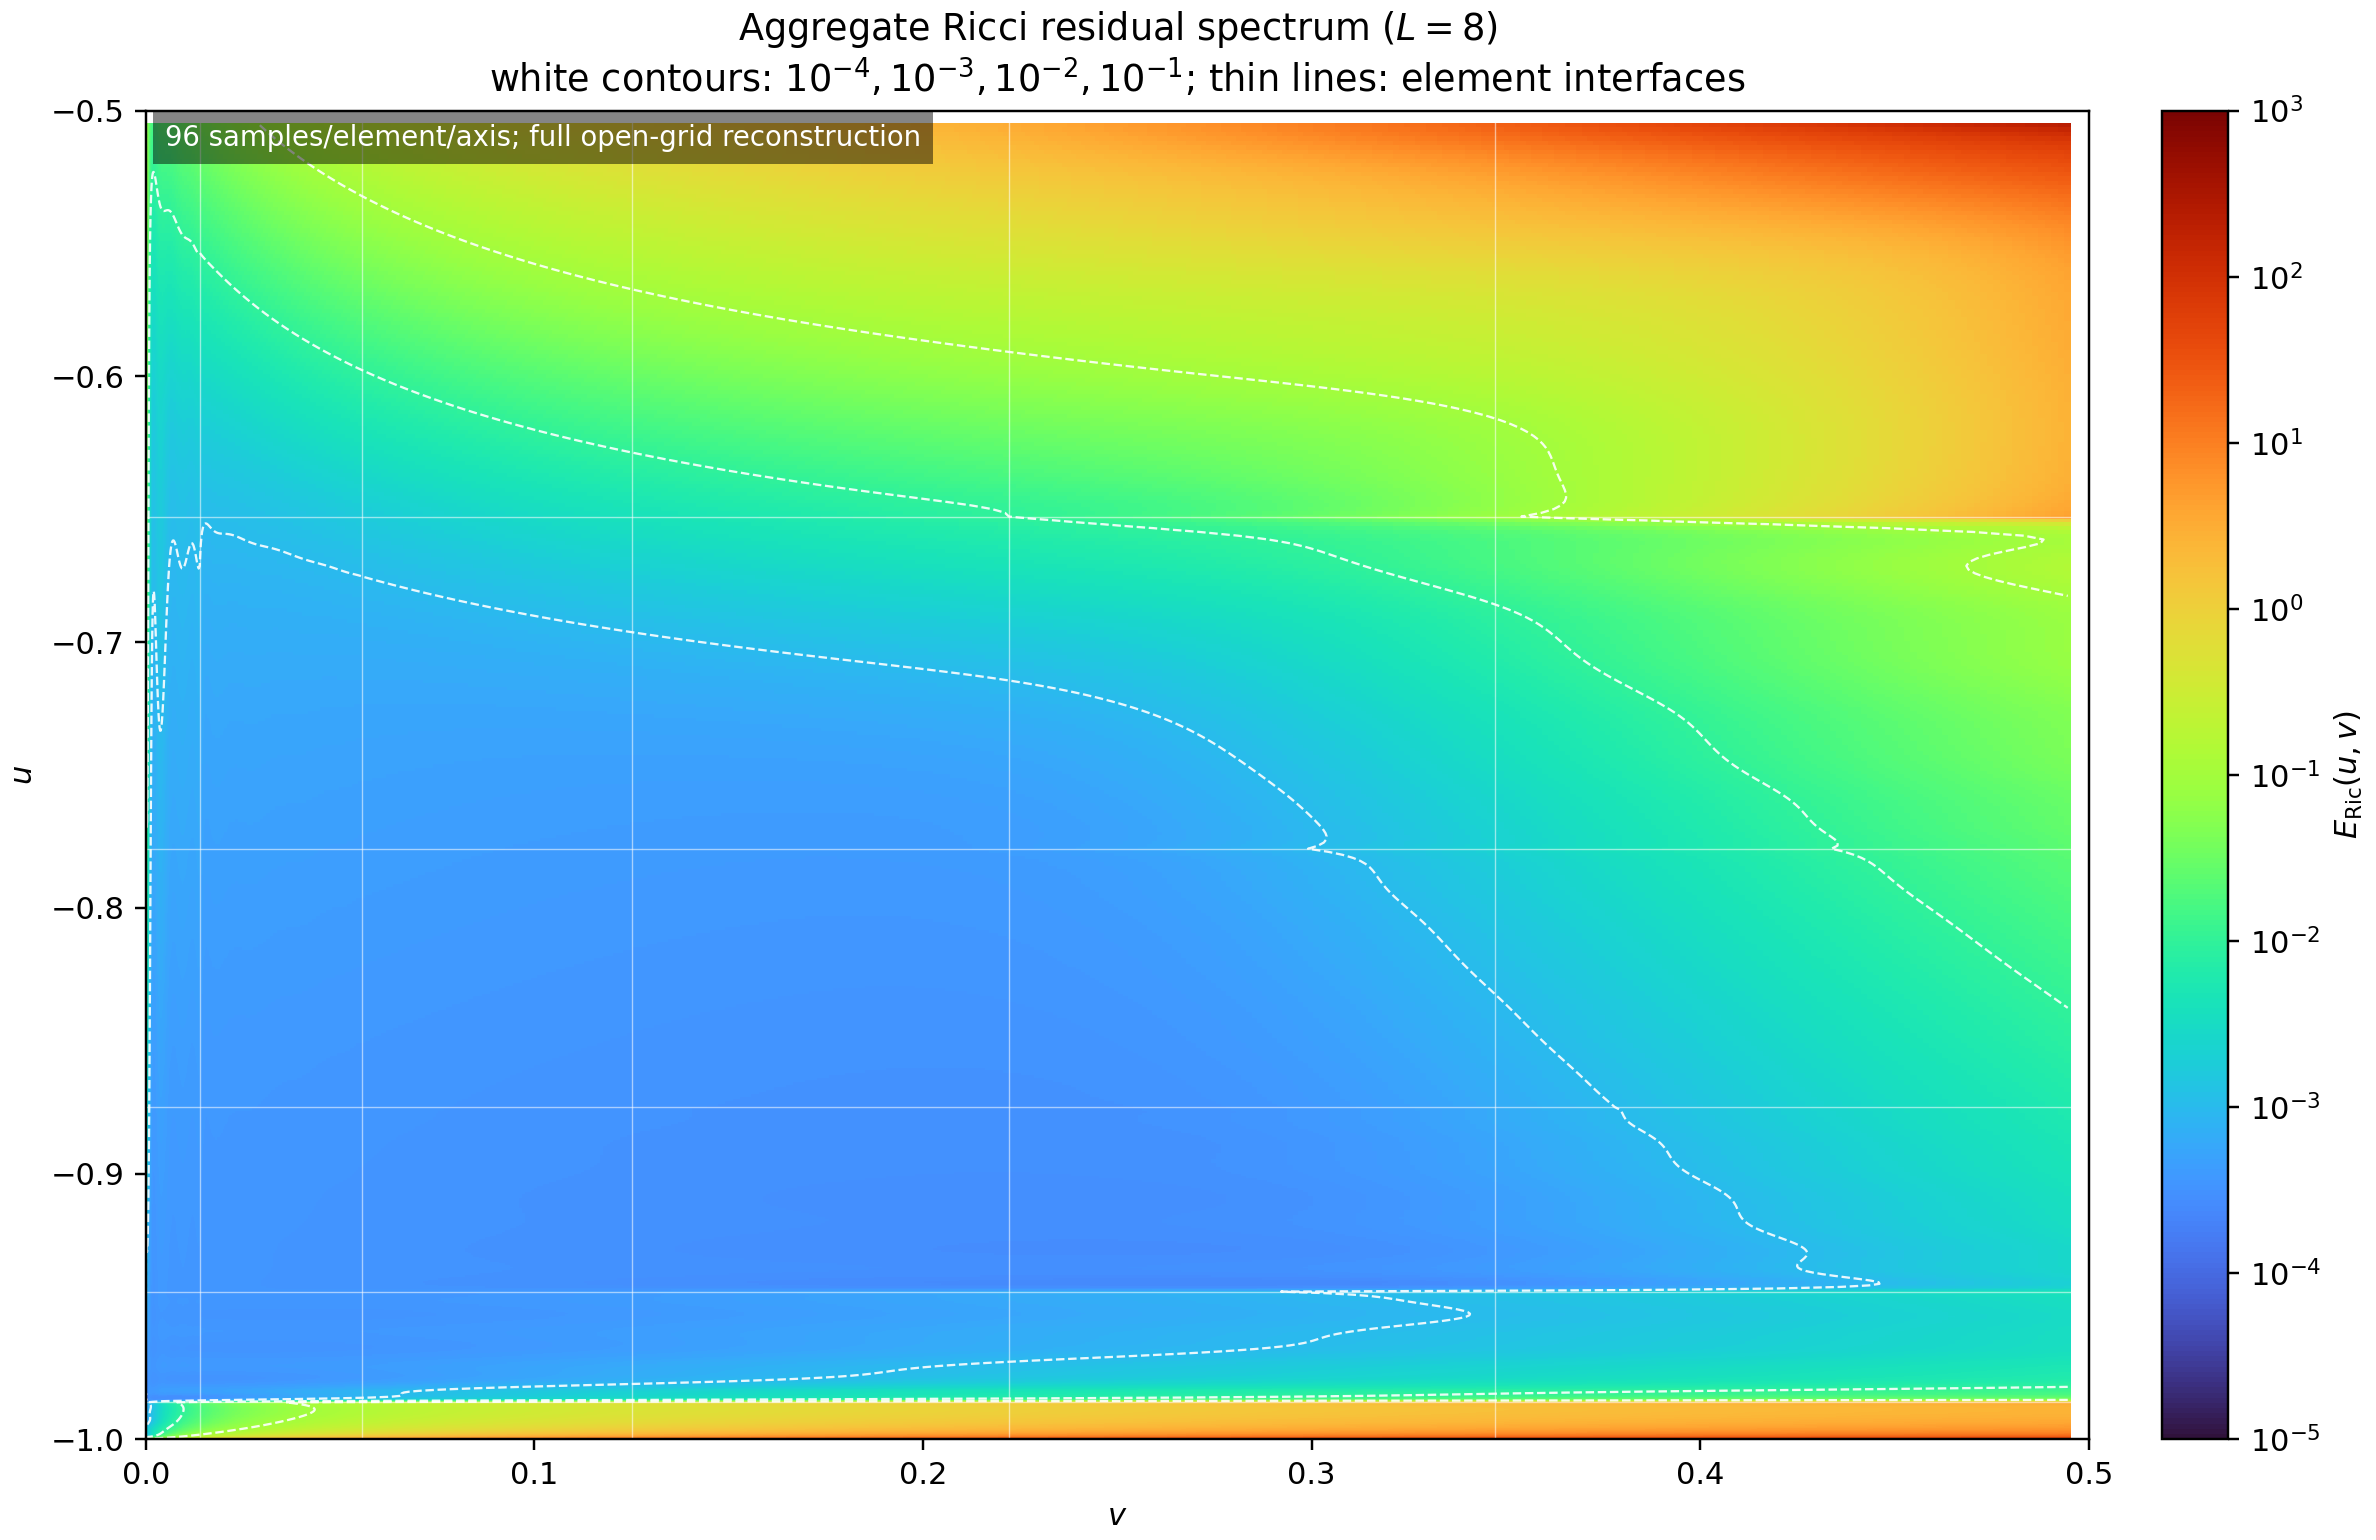
\includegraphics[width=0.8\textwidth]{
    ../experiments/exp05/results/residual-spectrum.png}
  \caption{Spectrum of the aggregate Ricci residual
  $E_{\mathrm{Ric}}(u,v)$.  Colors show the elementwise spectral
  interpolation of $\log_{10}E_{\mathrm{Ric}}$ on the open coordinate
  grid; white contours mark $10^{-4}$, $10^{-3}$, $10^{-2}$, and $10^{-1}$,
  and the thin lines are coordinate-element interfaces.}
  \label{fig:results-exp5-residual-spectrum}
\end{figure}

Figure \ref{fig:results-exp5-residual-spectrum} includes the unprotected
layers of the open grid.  The extreme null-curvature components can diverge
at the initial corner, but they are not differentiated to obtain this
residual.  The large unprotected values instead expose errors in the
first-order differentiation near the fractional-power endpoints and element
interfaces.  They are not used as an interior accuracy statistic; the
protected values are reported in Table~\ref{tab:results-exp5-residual}.

% \clearpage
